\section{Results and discussion}\label{sec:resultados}

This section presents the results obtained with the optimization framework described in Section~\ref{sec:metodologia}, applied to a matrix of roundwood timber bridge configurations for single-lane rural roads.
The matrix combines four design spans with the five native-forest timber strength classes of \textcite{NBR7190-1:2022}, keeping the roadway width, the design vehicle and all code coefficients fixed, so that the observed differences arise exclusively from the span and the strength class.

The presentation is organized in four parts.
The first describes the computational framework (Section~\ref{sec:plataforma}) and defines the case matrix (Section~\ref{sec:casos}).
The second details a reference cell of the matrix (Section~\ref{sec:caso_detalhado}), in which all analytical features of the tool are exercised, namely hypervolume convergence, efficient front, utilization of the checks, cost of robustness, global Sobol sensitivity and dispersion of the design variables.
The third covers the complete matrix (Section~\ref{sec:varredura}) and converts the results into preliminary design charts (Section~\ref{sec:abacos}).
The fourth fits a closed-form pre-sizing equation to the database of the parametric sweep (Section~\ref{sec:equacao}), as a numerical alternative to the graphical reading of the charts.


\subsection{Computational framework}\label{sec:plataforma}

The analysis and optimization framework described in Section~\ref{sec:metodologia} was implemented in an open-access computational platform for the design of timber bridges, capable of performing the complete verification of the structural members in accordance with \textcite{NBR7190-1:2022} and \textcite{nbr7188} \parencite{ReliaBridge2026}.
For each processed solution, the platform provides the efficient front, the verification report and the descriptive statistics of the design variables, serving as an instrument for implementing and transferring the results of this work to the designer.

\subsection{Definition of the case study matrix}\label{sec:casos}

The geometric, loading and code parameters kept constant across the whole matrix are presented in Table~\ref{tab:parametros}.
The 4.5~m roadway width corresponds to the usual cross-section of a single-lane rural road bridge, compatible with one vehicle at a time and with side wheel guards.

\begin{table}[!ht]
\caption{Geometric, loading and code parameters common to the whole matrix.\label{tab:parametros}}
\begin{threeparttable}
\begin{tabular*}{\columnwidth}{@{\extracolsep\fill}lc@{\extracolsep\fill}}
\toprule
Parameter & Value \\
\midrule
Roadway width, $b_{w,\mathrm{pista}}$ (cm) & 450 \\
Design vehicle (ABNT NBR 7188) & TB-240 \\
Wheel load, $p_{rodak}$ (kN) & 40 \\
Distributed variable load, $p_{qk}$ (kPa) & 4 \\
Distributed permanent load (wheel tracks), $p_{gk}$ (kPa)\tnote{a} & 0.10 \\
Axle spacing, $a$ (m) & 1.5 \\
Load-duration class & Short-term \\
Timber type & Natural timber \\
Moisture class & 3 \\
Partial factor for permanent actions, $\gamma_g$ & 1.30 \\
Partial factor for variable actions, $\gamma_q$ & 1.50 \\
Material partial factor (normal stresses), $\gamma_{wf}$ & 1.40 \\
Material partial factor (shear), $\gamma_{wc}$ & 1.80 \\
Quasi-permanent combination factor, $\psi_2$ & 0.30 \\
Creep coefficient, $\varphi$ & 0.80 \\
Robustness deviation, $\rho$ (\%) & 5.0 \\
\bottomrule
\end{tabular*}
\begin{tablenotes}
\footnotesize
\item[a] The self-weight of the deck and girders is computed internally by the platform from the geometry and the timber density. The permanent load $p_{gk}$ represents only the superimposed action of the wheel tracks, that is, the longitudinal running boards that guide the wheels.
This contribution was estimated from two $5 \times 30$~cm boards with a density of 620~kg/m\textsuperscript{3} ($\gamma \approx 6.1$~kN/m\textsuperscript{3}), resulting in about 0.18~kN/m along the span, or approximately 0.04~kPa when distributed over the roadway width.
A value of 0.10~kPa was adopted, rounded up to cover fastenings and the higher density usual for running boards.
\item The mechanical properties of the timber are not listed in this table because they vary among the cells of the matrix. They are those of Table~\ref{tab:classes_madeira}, according to the strength class of each cell.
\end{tablenotes}
\end{threeparttable}
\end{table}

The case matrix is the Cartesian product of four design spans and five strength classes, totalling twenty configurations, as shown in Table~\ref{tab:matriz}.
The span range of 3.0 to 6.0~m was chosen for two reasons.
The first is representativeness, since it corresponds to the usual width of the watercourses crossed by roundwood bridges on rural roads.
The second is formulation consistency, since within this interval the bending moment due to the moving load is given entirely by Eq.~\eqref{eq:mqk30}, without the additional crowd load term of Eq.~\eqref{eq:mqk45}, so that the result curves show no formulation discontinuity.

\begin{table}[!ht]
\caption{Case study matrix. Each cell corresponds to an independent NSGA-II run.\label{tab:matriz}}
\begin{threeparttable}
\begin{tabular*}{\columnwidth}{@{\extracolsep\fill}lccccc@{\extracolsep\fill}}
\toprule
 & \multicolumn{5}{c}{Strength class (ABNT NBR 7190-3)} \\
\cmidrule{2-6}
Span $L$ (m) & D20 & D30 & D40 & D50 & D60 \\
\midrule
3.0 & C-01 & C-02 & C-03 & C-04 & C-05 \\
4.0 & C-06 & C-07 & C-08 & C-09 & C-10 \\
5.0 & C-11 & C-12 & \textbf{C-13} & C-14 & C-15 \\
6.0 & C-16 & C-17 & C-18 & C-19 & C-20 \\
\bottomrule
\end{tabular*}
\begin{tablenotes}
\footnotesize
\item Cell C-13 ($L = 5.0$~m, class D40), highlighted in bold, is adopted as the reference case for the detailed analysis of Section~\ref{sec:caso_detalhado}.
\end{tablenotes}
\end{threeparttable}
\end{table}

The search bounds of the five design variables, common to all cells, are presented in Table~\ref{tab:intervalos}.
The bounds were set to cover the usual commercial dimensions of roundwood and sawn planks, without artificially restricting the search space of the algorithm.

\begin{table}[!ht]
\caption{Bounds adopted for the design variables.\label{tab:intervalos}}
\begin{threeparttable}
\begin{tabular*}{\columnwidth}{@{\extracolsep\fill}lcc@{\extracolsep\fill}}
\toprule
Variable & Minimum value (cm) & Maximum value (cm) \\
\midrule
Girder diameter, $d$ & 20 & 100 \\
Deck plank width, $b_w$ & 20 & 50 \\
Deck plank height, $h$ & 5 & 15 \\
Spacing between girders, $esp_{long}$ & 30 & 200 \\
Spacing between deck planks, $esp_{tab}$ & 2 & 5 \\
\bottomrule
\end{tabular*}
\end{threeparttable}
\end{table}

\subsection{Detailed reference case: $L = 5.0$~m, class D40}\label{sec:caso_detalhado}

This section exercises all analytical features of the platform on a single cell of the matrix, C-13.
The choice falls on an intermediate span and an intermediate strength class, so that the observed behaviour is representative of the whole set.
The results of the remaining nineteen cells are reported in condensed form in Section~\ref{sec:varredura}.

\subsubsection{Convergence of the optimization}\label{sec:hipervolume}

The quality of an approximated front is assessed, independently of visual inspection, by the hypervolume indicator ($HV$), which measures the portion of the objective space dominated by the front with respect to a reference point $\mathbf{r}$, according to Eq.~\eqref{eq:hv} \parencite{blank2020}.

\begin{equation}
HV(\mathcal{F}_1, \mathbf{r}) = \mathrm{Vol}\left(\bigcup_{\mathbf{x} \in \mathcal{F}_1} \left[f_1(\mathbf{x}), r_1\right] \times \left[f_2(\mathbf{x}), r_2\right]\right)
\label{eq:hv}
\end{equation}

The objectives are normalized by the ideal and nadir points observed over the whole run, so that the indicator is dimensionless and comparable across cells of different scales, and the reference point $r_1 = r_2 = 1.1$ is adopted in this normalized space.
Fig.~\ref{fig:convergencia_hv} shows the evolution of the hypervolume with the number of generations for cell C-13.

\begin{figure}[!ht]
    \centering
    
\includegraphics[width=0.45\textwidth]{figuras/en/convergencia_hv.png}
    \caption{Evolution of the hypervolume over the NSGA-II generations.}
    \label{fig:convergencia_hv}
\end{figure}

The curve shows a steep increase in the first twenty generations and asymptotic refinement thereafter, stabilizing at generation 40, which confirms the convergence of the optimization with the number of generations adopted in Table~\ref{tab:nsga2}.
Across the twenty cells of the matrix, stabilization occurs between generations 21 and 153, always before the 300 generations executed.
The spacing of the front, which measures the variation of the distance between neighbouring solutions, was low over the whole matrix, between 0.0136 and 0.0203, which ensures a uniform distribution of the solutions along the front.

\subsubsection{Efficient front and representative solutions}\label{sec:fronteira_ref}

The robust multi-objective optimization of cell C-13, with $\rho = 5\%$, produced a set of non-dominated solutions distributed along the efficient front shown in Fig.~\ref{fig:fronteira_ref}.
Table~\ref{tab:solucoes_ref} lists a representative sample of these solutions, with the corresponding objective functions and the largest value among the six limit state functions, confirming compliance with the code criteria even under the robust evaluation.

\begin{figure}[!ht]
    \centering
    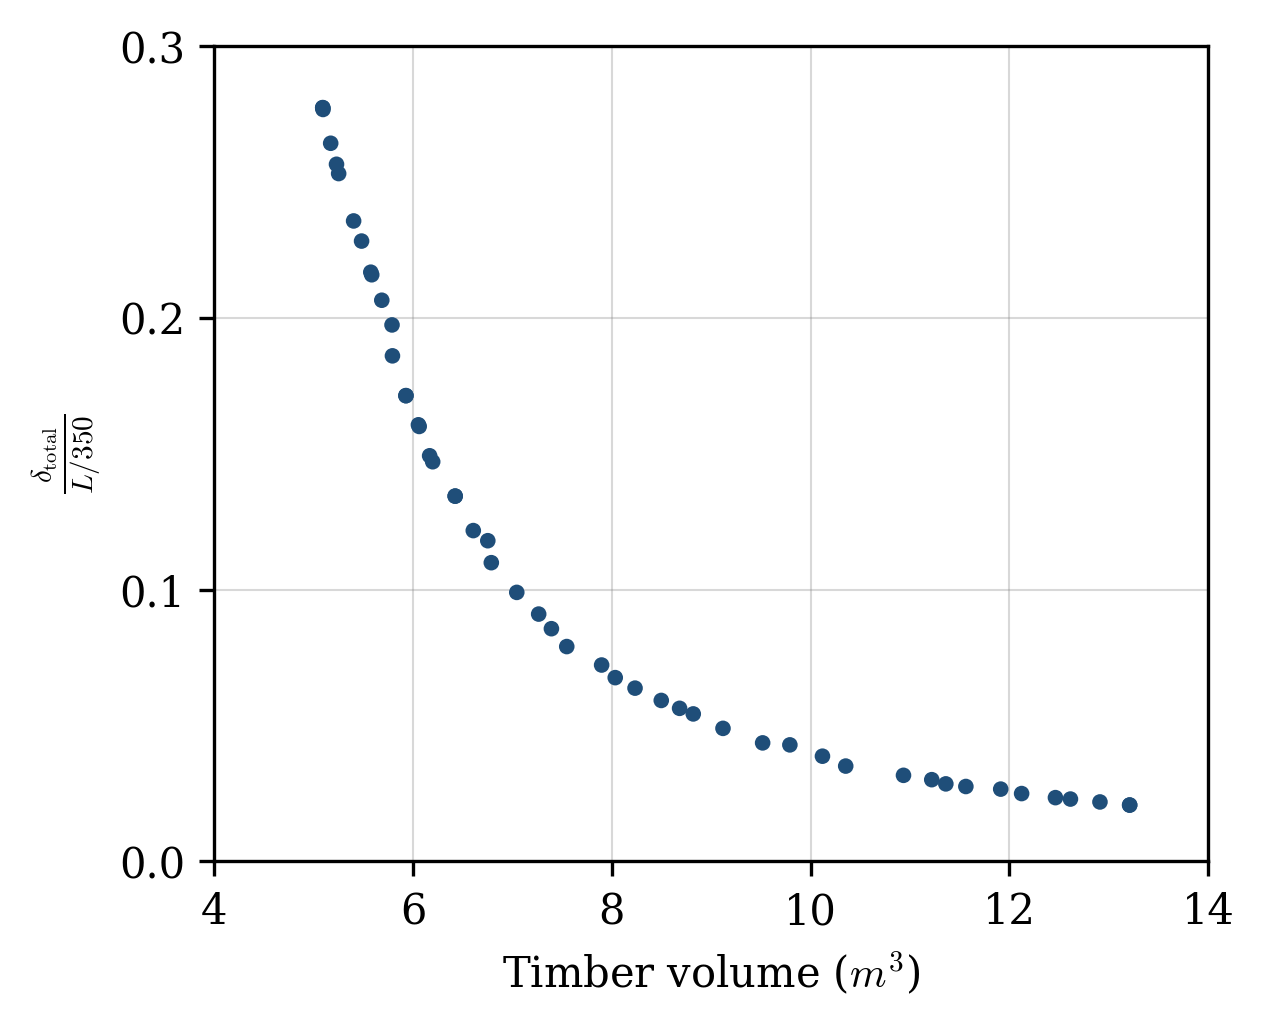
\includegraphics[width=0.6\textwidth]{figuras/en/pareto_frontier_C13.png}
    \caption{Efficient front of reference cell C-13 ($L = 5.0$~m, D40, $\rho = 5\%$).}
    \label{fig:fronteira_ref}
\end{figure}

\begin{table}[!ht]
\caption{Representative solutions of the efficient front of cell C-13.\label{tab:solucoes_ref}}
\begin{threeparttable}
\setlength{\tabcolsep}{3pt}
\begin{tabular*}{\textwidth}{@{\extracolsep{\fill}}cccccccc@{\extracolsep{\fill}}}
\toprule
$d$ (cm) & $b_w$ (cm) & $h$ (cm) & $esp_{long}$ (cm) & $esp_{tab}$ (cm) & $V_{\mathrm{total}}$ (m\textsuperscript{3}) & $\delta_{\mathrm{tot}}/(L/350)$ & $g_{\max}$ \\
\midrule
47.78 & 45.51 & 7.34 & 69.98 & 2.24 & 5.09 & 0.2772 & $-0.0018$ \\
51.01 & 45.50 & 7.26 & 67.89 & 4.73 & 5.57 & 0.2167 & $-0.0431$ \\
56.41 & 45.50 & 11.29 & 110.54 & 4.69 & 6.06 & 0.1600 & $-0.0012$ \\
64.15 & 45.55 & 10.71 & 97.85 & 4.98 & 7.04 & 0.0990 & $-0.0471$ \\
75.71 & 45.50 & 10.09 & 92.98 & 2.55 & 8.82 & 0.0543 & $-0.0759$ \\
90.92 & 45.50 & 7.93 & 58.55 & 2.57 & 11.36 & 0.0285 & $-0.0959$ \\
100.00 & 45.50 & 6.99 & 81.23 & 4.53 & 13.21 & 0.0208 & $-0.0002$ \\
\bottomrule
\end{tabular*}
\begin{tablenotes}
\footnotesize
\item Seven solutions extracted from the final front of 50 non-dominated points, ordered from the minimum timber volume end (first row) to the minimum dimensionless deflection end (last row), including both ends. $g_{\max}$ is the largest value among the strength and serviceability limit state functions $g_1$ to $g_4$ of the solution, and it is negative in all rows, which confirms feasibility under the robust evaluation.
The geometric limit state functions $g_5$ and $g_6$, which only check that the spacings fall within the bounds of Table~\ref{tab:intervalos}, are excluded from this maximum because they do not express a structural margin.
\end{tablenotes}
\end{threeparttable}
\end{table}

The front extends from 5.09~m\textsuperscript{3} of timber, with a total deflection equal to 27.7\% of the code limit, to 13.21~m\textsuperscript{3}, with a deflection of only 2.1\% of the limit.
The two objectives therefore vary on different scales. The volume slightly more than doubles (2.6 times), whereas the dimensionless deflection drops about thirteen times.
This imbalance is a direct manifestation of the geometry of the circular section.
Along the front, the volume grows approximately with $d^{1.28}$, whereas the deflection decreases with $d^{-3.54}$, so that the joint fit gives $\delta_{\mathrm{tot}}/(L/350) \propto V^{-2.76}$, with a coefficient of determination of 0.995.
In design terms, this means that the first additional cubic metres of timber buy a substantial reduction in displacement. Doubling the volume from the economical end already reduces the deflection by about seven times, and doubling it again would reduce this value by a similar additional factor, although the studied front does not cover this second doubling.

The useful part of the front for the designer is therefore concentrated in the first half of the volume range. At 7.90~m\textsuperscript{3}, about one third of the way between the ends, the deflection already drops to 7.2\% of the limit. Beyond this point the marginal return falls, and going from $V = 8.82$~m\textsuperscript{3} to $V = 13.21$~m\textsuperscript{3} (an increase of 49.5\%) reduces the deflection from only 5.4\% to 2.1\% of the limit, a gain of slightly more than three percentage points over an already ample margin. Increasing the volume beyond the first third of the front is therefore no longer justified in practice.


The active constraint along the front is the same from end to end.
Deck bending ($g_4$) is the check closest to its limit in all 50 solutions of the front, without exception, including the minimum volume end, where it practically saturates at the code limit ($g_{\max} \approx 0$, utilization of 99.8\%).
Girder bending ($g_1$) follows closely at this same end, with a utilization of 99.7\%, but does not overtake the deck as the governing constraint at any point of the front in this version of the matrix, which nevertheless confirms how close the two checks remain to each other.
It can therefore be stated that moving along the front means increasing the girder diameter, which quickly gains margin, while the deck remains anchored at its limit throughout the whole trade-off space.
The deck is thus not a secondary element of the design but the element that limits performance. The width-height pair of the plank and the girder spacing define the local bending span under the wheel, and they dictate the shape of the curve in Fig.~\ref{fig:fronteira_ref}.

\subsubsection{Utilization of the code checks}\label{sec:utilizacao}

Fig.~\ref{fig:utilizacao} presents the utilization of each code check for a selected solution of the front, understood as the ratio between demand and resistance for the ultimate limit states, or between displacement and allowable limit for the serviceability limit state.
A value of 100\% corresponds to the code limit.
Since the limit state functions are normalized in the form $g_j = (S_j - R_j)/R_j$, the utilization follows directly from them as $(1 + g_j)\times 100\%$.
The solution analysed is the minimum timber volume solution of the front, the first row of Table~\ref{tab:solucoes_ref}, as it is of immediate interest for preliminary design.

\begin{figure}[!ht]
    \centering
    
\includegraphics[width=0.65\textwidth]{figuras/en/utilizacao_C13.png}
    \caption{Utilization of each code check for the selected solution of the robust front of cell C-13.}
    \label{fig:utilizacao}
\end{figure}

The economical solution of cell C-13 shows two practically saturated checks and two with a relevant margin.
Deck bending governs the design, with a utilization of 99.8\%, consistent with the $g_{\max} \approx 0$ recorded in the first row of Table~\ref{tab:solucoes_ref}.
Immediately behind comes girder bending, at 99.7\%.
The two bending checks therefore become active almost simultaneously, which is the signature of a well-balanced design, since the algorithm could not reduce the volume further without violating one of them while the other was still at its limit.

The margins are concentrated in the remaining checks, although unevenly.
Girder deflection ($g_3$, which combines the quasi-permanent $L/350$ and characteristic $L/500$ limits) operates at 77.7\% of its combined limit, and shear at only 44.9\% of the design strength, the latter being the check with the largest reserve.

For the 5~m span, D40 timber and the TB-240 design vehicle, the design remains governed by bending strength rather than stiffness, but the deflection margin is no longer as wide as in the other cells. Section~\ref{sec:varredura} shows that, for stiffer classes at the same span or for longer spans, this same check comes close to governing.
The ample shear margin results from the circular geometry, in which the section area grows with $d^2$ while the shear demand is independent of the diameter, and indicates that the shear check, traditionally cited as critical for short roundwood members, is not decisive in this span range.


\subsubsection{Cost of robustness}\label{sec:custo_robustez}

Deterministic optimization tends to place the optimal solutions exactly on the boundary of the active constraints, making them sensitive to small variations in the design variables.
In roundwood timber bridges, this sensitivity is aggravated by the natural variability of the member diameter and by manufacturing and assembly tolerances.
The incorporation of robustness shifts the efficient front into the interior of the feasible domain, penalizing solutions with a practically zero girder bending limit state function ($g_1 \approx 0$), since under a perturbation of $\pm\rho$ part of the realizations would violate it.

To quantify this effect, cell C-13 was re-optimized for five deviation levels on a uniform grid, $\rho \in \{0\%,\ 5\%,\ 10\%,\ 15\%,\ 20\%\}$, keeping all other algorithm parameters unchanged (Table~\ref{tab:nsga2}).
The case $\rho = 0\%$ corresponds to deterministic optimization, with $N_c = 1$, and serves as the reference.
The grid was extended up to $\rho = 20\%$, well beyond the design value of 5\% adopted in the rest of the matrix, to characterize the relationship between $\rho$ and the volume cost over a wider range than strictly needed for design.
The comparison is made at a single point of each front, the minimum volume solution (the end of immediate interest for preliminary design), rather than over paired ranges of dimensionless deflection, a reading discarded because it is sensitive to the noise of a single independent NSGA-II run per $\rho$ level.

\begin{figure}[!ht]
    \centering
    
\includegraphics[width=0.7\textwidth]{figuras/en/custo_robustez_C13.png}
    \caption{Efficient fronts of cell C-13 for $\rho = 0\%$, $5\%$, $10\%$, $15\%$ and $20\%$.}
    \label{fig:custo_robustez}
\end{figure}

\begin{table}[!ht]
\caption{Minimum volume of the efficient front of cell C-13 for each deviation level $\rho$, and percentage increase with respect to the deterministic case ($\rho = 0\%$).\label{tab:custo_robustez}}
\begin{threeparttable}
\begin{tabular*}{\columnwidth}{@{\extracolsep\fill}ccc@{\extracolsep\fill}}
\toprule
$\rho$ (\%) & $V_{\min}$ (m\textsuperscript{3}) & $\Delta$ \\
\midrule
0.0 & 4.800 & -- \\
5.0 & 5.090 & $+6.0\%$ \\
10.0 & 5.414 & $+12.8\%$ \\
15.0 & 5.788 & $+20.6\%$ \\
20.0 & 6.091 & $+26.9\%$ \\
\bottomrule
\end{tabular*}
\begin{tablenotes}
\footnotesize
\item $V_{\min}$ is the volume of the minimum timber volume solution of the efficient front at that $\rho$ level. $\Delta$ is the percentage increase with respect to $V_{\min}(\rho{=}0\%)$.
\end{tablenotes}
\end{threeparttable}
\end{table}

Fig.~\ref{fig:custo_robustez} shows the five fronts shifting visibly and orderly into the interior of the feasible domain as $\rho$ increases.
At the minimum volume end, Table~\ref{tab:custo_robustez} shows a monotonic increase approximately proportional to $\rho$, from 4.800~m\textsuperscript{3} in the deterministic case to 5.090~m\textsuperscript{3} ($+6.0\%$) at $\rho = 5\%$, 5.414~m\textsuperscript{3} ($+12.8\%$) at $\rho = 10\%$, 5.788~m\textsuperscript{3} ($+20.6\%$) at $\rho = 15\%$ and 6.091~m\textsuperscript{3} ($+26.9\%$) at $\rho = 20\%$.
The marginal cost rate increases slightly with $\rho$, from about 1.2\% of additional volume per percentage point of $\rho$ between 0 and 5\% to about 1.3\% to 1.4\% per percentage point at the higher levels of the grid.

The value $\rho = 5\%$ remains the default across the whole matrix (Section~\ref{sec:varredura}) for consistency with the literature on dimensional tolerances of roundwood members.

\subsubsection{Global sensitivity analysis by Sobol indices}\label{sec:sobol}

To identify which design variables most influence the violation of each constraint under perturbation, a global sensitivity analysis was performed with the Sobol method \parencite{Sobol2001}, as implemented in the \texttt{UQpy} library \parencite{Olivier2020}. The total-effect indices $S_{T_i}$ of the five design variables were estimated with respect to the six limit state functions, from an independent sample of $N = 20\,000$ points over the domain of each variable (Table~\ref{tab:intervalos}). This sample size was defined from preliminary convergence tests, in which the variation of the Sobol indices was below 1\% when the sample size was doubled.

\begin{figure}[!ht]
    \centering
    
\includegraphics[width=0.85\textwidth]{figuras/en/sobol_heatmap_C13.png}
    \caption{Total-effect Sobol indices ($S_{T_i}$) of the design variables on the constraints, cell C-13.}
    \label{fig:sobol}
\end{figure}

\begin{table}[!ht]
\caption{Most influential variable (dominant $S_{T_i}$) per constraint.\label{tab:sobol}}
\begin{threeparttable}
\footnotesize
\setlength{\tabcolsep}{3pt}
\begin{tabular*}{\columnwidth}{@{\extracolsep\fill}lccc@{\extracolsep\fill}}
\toprule
Constraint & Dominant variable & $S_{T_i}$ & Share \\
\midrule
$g_1$: girder bending & $d$ & 1.005 & 98.2\% \\
$g_2$: girder shear & $d$ & 1.021 & 96.0\% \\
$g_3$: girder deflection & $d$ & 1.003 & 97.2\% \\
$g_4$: deck bending & $esp_{long}$ & 4.964 & 93.0\% \\
$g_5$: girder spacing & $esp_{long}$ & 1.003 & 100.0\% \\
$g_6$: deck plank spacing & $esp_{tab}$ & 1.000 & 100.0\% \\
\bottomrule
\end{tabular*}
\begin{tablenotes}
\footnotesize
\item The relative share is the fraction of the sum of the total-effect indices of the five variables for that constraint, computed after truncating negative estimates at zero.
The total-effect indices are estimated by variance differences and are therefore not bounded to the interval $[0,1]$ for strongly non-linear responses. The value of 4.964 associated with $g_4$ reflects the non-linearity introduced by rounding the integer number of members accommodated on the roadway.
\end{tablenotes}
\end{threeparttable}
\end{table}

The result confirms the mechanical expectation for the three girder constraints.
The diameter $d$ accounts for 98.2\% of the sensitivity of bending, 96.0\% of shear and 97.2\% of deflection, whereas the four remaining variables together account for less than 4\% in any of them.
This dominance is expected because $d$ is the only variable that enters simultaneously the area, the section modulus and the second moment of area of the circular section, and it is even more pronounced in the serviceability limit state, in which the second moment of area varies with $d^4$ while the area, which governs the self-weight, varies only with $d^2$.

Deck bending behaves differently and more informatively.
In this check, the diameter is practically irrelevant, with a share of 0.1\%, and the dominant variable becomes the girder spacing, with 93.0\%, followed by the plank height, with 4.4\%, and the plank width, with 2.5\%.
The girder spacing is the local bending span of the plank, in which the bending demand grows with the square of this span, whereas the plank resistance grows only with $b_w h^2$.
The girder spacing is therefore the coupling variable between the two subsystems of the superstructure. It does not affect the girder in isolation, but defines how much load reaches each girder and which span the deck must bridge.
The last two constraints are, by construction, exclusive functions of the respective spacings, and the analysis recovers them with a 100\% share, which serves as a consistency check of the estimator itself.

A hierarchy for possible execution controls in timber bridges can be identified here.
The diameter of the roundwood members and the girder spacing concentrate practically all the sensitivity of the system.
These are the variables that justify investment in strict dimensional control, the former at the stage of log selection and grading, with rejection of members outside the nominal range, and the latter at the assembly stage, with a positioning template for the girders.
The deck plank dimensions, $b_w$ and $h$, and the deck plank spacing, $esp_{tab}$, admit looser execution tolerances without measurable loss of safety, since they account for a small portion of the variability of the limit state functions.
This distinction is relevant for rural road construction, where quality control is necessarily selective and must be directed at what actually matters.

\subsubsection{Dispersion of the design variables along the front}\label{sec:dispersao}

As a complement to the quality indicators of the front in the objective space, Fig.~\ref{fig:boxplot} characterizes the diversity of the front in the decision space, showing the dispersion of each design variable among the non-dominated solutions.

\begin{figure}[!ht]
    \centering
    
\includegraphics[width=0.75\textwidth]{figuras/en/boxplot_variaveis_C13.png}
    \caption{Dispersion of the design variables along the efficient front of cell C-13.}
    \label{fig:boxplot}
\end{figure}

\begin{table}[!ht]
\caption{Descriptive statistics of the design variables on the efficient front of cell C-13.\label{tab:estatistica}}
\begin{threeparttable}
\footnotesize
\setlength{\tabcolsep}{3pt}
\begin{tabular*}{\textwidth}{@{\extracolsep{\fill}}lccccccccc@{\extracolsep{\fill}}}
\toprule
Variable & Mean & Std. dev. & CV (\%) & Minimum & $Q_1$ & Median & $Q_3$ & Maximum & Range \\
\midrule
$d$ (cm) & 68.84 & 17.14 & 24.90 & 47.78 & 54.49 & 64.89 & 82.72 & 100.00 & 52.22 \\
$b_w$ (cm) & 45.58 & 0.20 & 0.44 & 45.50 & 45.50 & 45.50 & 45.51 & 46.60 & 1.10 \\
$h$ (cm) & 9.13 & 1.64 & 17.92 & 6.99 & 7.34 & 9.36 & 10.68 & 11.39 & 4.40 \\
$esp_{long}$ (cm) & 87.64 & 17.90 & 20.43 & 58.55 & 69.50 & 91.99 & 103.23 & 120.72 & 62.17 \\
$esp_{tab}$ (cm) & 3.44 & 1.14 & 33.14 & 2.18 & 2.44 & 2.56 & 4.68 & 4.98 & 2.79 \\
\bottomrule
\end{tabular*}
\begin{tablenotes}
\footnotesize
\item Statistics computed over the 50 non-dominated solutions of the final front.
\end{tablenotes}
\end{threeparttable}
\end{table}

The dispersion is strongly uneven among the variables, both in absolute range and in relative variation.
The girder spacing is by far the variable with the largest range along the front, with 62.2~cm of variation, a coefficient of variation of 20.4\% and an interquartile range of 33.7~cm, covering a large part of the search domain of Table~\ref{tab:intervalos}.
Next comes the girder diameter, with a range of 52.2~cm and a coefficient of variation of 24.9\%.
These two variables are nevertheless the ones that build the trade-off between the two objectives, and no other variable comes close to them in absolute range.

At the opposite extreme, the deck plank width is practically invariant, with a coefficient of variation of 0.4\% and an interquartile range of only 0.01~cm around 45.5~cm.
The algorithm converges to this value regardless of the point of the front chosen by the designer, which has a direct practical consequence, since $b_w \approx 45.5$~cm can be fixed \textit{a priori} in preliminary design without a performance penalty, reducing the effective dimensionality of the decision from five to four.
The two remaining variables occupy intermediate positions, but with different readings. The plank height has a moderate coefficient of variation of 17.9\% (4.4~cm range), whereas the deck plank spacing has 33.1\% (2.8~cm range), much more dispersed, approaching the minimum admissible value of 2~cm at least at one point of the front (observed minimum of 2.18~cm, only 0.18~cm above the lower bound of the search domain).

The comparison with Section~\ref{sec:sobol} is convergent.
The two variables with the highest sensitivity are exactly the two with the largest absolute range on the front, and each one controls a subsystem, although their order is reversed depending on the indicator. The girder spacing is the variable with the largest range on the front and accounts for 93.0\% of the sensitivity of deck bending, whereas the diameter, second in range, accounts for 96 to 98\% of the sensitivity of the three girder checks.
Moving along the front therefore consists of adjusting these two parameters simultaneously, one per subsystem.
The three remaining variables, which combine low sensitivity and a small absolute range, behave as constructive parameters rather than decision variables. This suggests that a simplified preliminary design procedure could fix them and optimize only $d$ and $esp_{long}$ without significant loss of quality.

\subsection{Parametric sweep: effect of span and strength class}\label{sec:varredura}

This section reports the results of the twenty cells of the matrix.
For each cell, the minimum timber volume solution was extracted from the efficient front, as it is of immediate interest for preliminary design, and the corresponding dimensions, total volume, dimensionless deflection and governing check were recorded.
The consolidated results are given in Table~\ref{tab:resultados_matriz}.

\begin{table}[!ht]
\caption{Consolidated results of the parametric sweep, minimum timber volume solution of each cell of the matrix.\label{tab:resultados_matriz}}
\begin{threeparttable}
\footnotesize
\setlength{\tabcolsep}{3pt}
\begin{tabular*}{\textwidth}{@{\extracolsep{\fill}}llrrrrrrrrl@{\extracolsep{\fill}}}
\toprule
Cell & $L$ (m) / Class & $d$ & $b_w$ & $h$ & $esp_{long}$ & $esp_{tab}$ & $V_{\mathrm{total}}$ & $\delta_{\mathrm{tot}}/(L/350)$ & $g_{\max}$ & Governing \\
 & & (cm) & (cm) & (cm) & (cm) & (cm) & (m\textsuperscript{3}) & & & check \\
\midrule
C-01 & 3.0 / D20 & 43.30 & 38.59 & 6.41 & 49.35 & 4.24 & 2.988 & 0.0943 & $-0.0000$ & Deck bending \\
C-02 & 3.0 / D30 & 37.77 & 38.59 & 6.44 & 55.16 & 4.20 & 2.464 & 0.1364 & $-0.0000$ & Deck bending \\
C-03 & 3.0 / D40 & 34.50 & 39.44 & 6.05 & 59.94 & 4.92 & 2.154 & 0.1634 & $-0.0007$ & Deck bending \\
C-04 & 3.0 / D50 & 31.81 & 38.57 & 5.85 & 62.83 & 2.20 & 1.903 & 0.1992 & $-0.0000$ & Girder bending \\
C-05 & 3.0 / D60 & 30.12 & 38.58 & 5.57 & 64.70 & 5.00 & 1.745 & 0.2121 & $-0.0140$ & Deck bending \\
\midrule
C-06 & 4.0 / D20 & 52.37 & 26.72 & 5.00 & 32.20 & 2.84 & 5.089 & 0.1355 & $-0.0008$ & Girder bending \\
C-07 & 4.0 / D30 & 45.85 & 45.73 & 8.71 & 72.78 & 2.69 & 4.076 & 0.1988 & $-0.0000$ & Deck bending \\
C-08 & 4.0 / D40 & 43.05 & 40.00 & 8.43 & 75.64 & 4.81 & 3.695 & 0.2149 & $-0.0068$ & Deck bending \\
C-09 & 4.0 / D50 & 38.71 & 35.69 & 5.04 & 54.90 & 4.81 & 3.163 & 0.2775 & $-0.0003$ & Deck bending \\
C-10 & 4.0 / D60 & 36.47 & 45.65 & 7.14 & 112.05 & 4.09 & 2.845 & 0.3132 & $-0.0004$ & Deck bending \\
\midrule
C-11 & 5.0 / D20 & 60.13 & 45.51 & 8.07 & 54.32 & 4.23 & 7.331 & 0.1585 & $-0.0005$ & Girder bending \\
C-12 & 5.0 / D30 & 52.55 & 40.91 & 8.21 & 63.90 & 3.19 & 6.001 & 0.2277 & $-0.0001$ & Deck bending \\
\textbf{C-13} & 5.0 / D40 & 47.78 & 45.51 & 7.34 & 69.98 & 2.24 & 5.090 & 0.2772 & $-0.0018$ & Deck bending \\
C-14 & 5.0 / D50 & 44.49 & 45.50 & 10.89 & 125.17 & 4.61 & 4.562 & 0.3543 & $-0.0004$ & Girder bending \\
C-15 & 5.0 / D60 & 41.79 & 45.50 & 6.55 & 78.07 & 3.01 & 4.084 & 0.3581 & $-0.0011$ & Deck bending \\
\midrule
C-16 & 6.0 / D20 & 66.72 & 45.42 & 6.47 & 38.08 & 2.11 & 9.978 & 0.1740 & $-0.0002$ & Deck bending \\
C-17 & 6.0 / D30 & 58.17 & 45.42 & 12.74 & 106.87 & 4.84 & 7.907 & 0.2718 & $-0.0015$ & Girder bending \\
C-18 & 6.0 / D40 & 52.89 & 45.42 & 11.48 & 114.21 & 4.96 & 6.771 & 0.3333 & $-0.0003$ & Deck bending \\
C-19 & 6.0 / D50 & 49.24 & 45.43 & 10.55 & 119.44 & 2.45 & 6.015 & 0.3924 & $-0.0008$ & Deck bending \\
C-20 & 6.0 / D60 & 47.60 & 45.44 & 9.90 & 172.14 & 2.53 & 5.632 & 0.3914 & $-0.0000$ & Deck bending \\
\bottomrule
\end{tabular*}
\begin{tablenotes}
\footnotesize
\item All cells with $\rho = 5\%$ and the algorithm parameters of Table~\ref{tab:nsga2}.
The ``Governing check'' column records the constraint with the largest $g_j$ value among $g_1$ to $g_4$ in the reported solution, that is, the one closest to the code limit, and $g_{\max}$ is the corresponding value.
\end{tablenotes}
\end{threeparttable}
\end{table}

\paragraph{Effect of span.} Timber consumption grows more than proportionally with span in all classes, as expected, and the exponent of the power law $V \propto L^{n}$ fitted to the four observations of each class varies little among classes, between $n = 1.64$ (D40) and $n = 1.73$ (D20), with coefficients of determination of at least 0.996 in all cases.
The general trend is a decrease of the exponent from D20 to D40 ($n = 1.73$, 1.69 and 1.64), followed by a partial recovery in the next two classes ($n = 1.67$ for D50 and $n = 1.68$ for D60), without strict monotonicity across the matrix.
In absolute terms, going from 3.0 to 6.0~m multiplies consumption by 3.3 for class D20 and by 3.2 for class D60, a much narrower range than the differences between the governing checks of each class would suggest.
The coupling between self-weight and performance, stronger in the lower strength classes, remains present as a mechanism, but its effect on the exponent is small in this span range.

\paragraph{Effect of strength class.} In this matrix, the volume reduction obtained by moving up in class is approximately uniform across the four spans. Going from D20 to D60, consumption drops by 41.6\% for the 3~m span, 44.1\% for 4~m, 44.3\% for 5~m and 43.6\% for 6~m.
Contrary to what a matrix with a more restricted search domain might suggest, none of the twenty cells saturates at the $d = 20$~cm lower bound of Table~\ref{tab:intervalos}. Even the most economical cell, C-05 (3~m, D60), converges to $d = 30.1$~cm, above the bound.
The table instead reveals a pattern of uniformly tight structural convergence. In all twenty cells the minimum volume solution operates with at most 1.40\% margin on the governing check ($g_{\max}$ between $-0.0140$ and $-0.0000$), with no relevant margin in any of them. The largest margin occurs in C-05 (3~m, D60) and the second largest in C-08 (4~m, D40, $g_{\max} = -0.0068$), with no clear systematic pattern between span and margin.
This uniformity is the expected outcome of a well-converged algorithm exploring a continuous search domain, and it replaces the dimensional saturation effect that a narrower diameter range would produce.

For all spans, the first class upgrade is the most effective, by a considerable margin.
Going from D20 to D30 reduces consumption by between 17.5\% (3~m span) and 20.8\% (6~m span), accounting alone for 41\% to 48\% of the total saving between D20 and D60, whereas the subsequent upgrades individually yield between 3.8\% and 12.4\% of the D20 volume.
The flattening in the subsequent steps is caused by the trade-off identified in the problem formulation. Between D20 and D60 the characteristic bending strength triples and the modulus of elasticity almost doubles, but the density also doubles, from 500 to 1000~kg/m\textsuperscript{3}, and the added self-weight consumes part of the strength gain.
The gain neither vanishes nor reverses within the studied range, so that, strictly speaking, there is no optimal class in the sense of an interior minimum.
From a preliminary design standpoint, the recommendation derived from the matrix is that specification efforts should concentrate on guaranteeing at least class D30, for any of the four spans, and that the pursuit of higher classes is justified only when high-class timber is available without a relevant cost premium.

The matrix is fully monotonic, which is the expected consistency check, since within each class the volume increases with span and within each span it decreases from class D20 to D60, without a single inversion among the twenty cells.

\paragraph{Governing check.} Bending governs the entire matrix. Fifteen of the twenty cells are governed by deck bending and the remaining five by girder bending, with no cell governed by deflection.
The two bending checks alternate across the matrix without a clear pattern in span or class, consistent with what Section~\ref{sec:fronteira_ref} shows for the reference cell.
The girder deflection check ($g_3$), although never governing, comes extremely close to its limit in three cells with the most severe span and class, with utilizations of 99.21\% in C-15 ($L = 5.0$~m, D60), 99.90\% in C-19 ($L = 6.0$~m, D50) and 99.97\% in C-20 ($L = 6.0$~m, D60), always a few hundredths of a percentage point behind deck bending.
The narrowest near-tie occurs in C-20, in which deck bending ($g_4 = -0.0000$, utilization of 100.00\%) and girder deflection (99.97\%) differ by less than three hundredths of a percentage point, and C-19 repeats the pattern, with the deck at 99.92\% against deflection at 99.90\%, decided by the fourth decimal place.

The predominance of the deck has a mechanical origin in the coupling through the girder spacing.
Since the circular section becomes more volume-efficient as its diameter increases, the algorithm concentrates the material in a few girders and spreads them apart until the moment under the wheel, which grows with the local span of the plank (Eq.~\eqref{eq:mqktab}), exhausts the capacity of the deck.

The practical consequence remains essentially the same, with a relevant caveat for the most severe classes and spans of the matrix.
In roundwood timber bridges within this span range, under the TB-240 vehicle, bending strength rather than stiffness governs the entire matrix. The quasi-permanent index $\delta_{\mathrm{tot}}/(L/350)$ remains below 39.3\% in all twenty cells (maximum of 0.392 in C-19).
The characteristic (rare) combination ($L/500$, without creep), however, already approaches its limit for the higher strength classes and longer spans, becoming nearly active in C-15, C-19 and C-20. This is a warning that, for spans or classes beyond those studied here, the transition from strength to stiffness governance may occur earlier than the isolated reading of the quasi-permanent index would suggest.

Shear, in turn, remains far from its limit throughout the matrix, with a maximum utilization of 60.2\%. The area of the circular section grows with $d^2$ while the shear demand is independent of the diameter, so that this check, traditionally cited as critical for short roundwood members, does not approach its limit even after the correction of Eq.~\eqref{eq:qqkenv} for short spans.

\subsection{Preliminary design charts}\label{sec:abacos}

The results of Table~\ref{tab:resultados_matriz} were converted into direct-reading design charts, intended for use by the designer at the conceptual stage, before any computational processing.
Fig.~\ref{fig:abaco_volume} presents the total timber volume as a function of span, with one curve per strength class. Fig.~\ref{fig:abaco_volume_m2} normalizes this volume by the deck area, allowing direct comparison between spans. Fig.~\ref{fig:abaco_diametro} provides the required girder diameter, which is the most immediate procurement information for the engineering design.

\begin{figure}[!ht]
    \centering
    \begin{subfigure}{0.40\textwidth}
        \centering
        
\includegraphics[width=\textwidth]{figuras/en/abaco_volume_vs_vao.png}
        \caption{Total timber volume as a function of the design span.}
        \label{fig:abaco_volume}
    \end{subfigure}
    \hfill
    \begin{subfigure}{0.40\textwidth}
        \centering
        
\includegraphics[width=\textwidth]{figuras/en/abaco_volume_por_m2.png}
        \caption{Timber consumption per square metre of deck.}
        \label{fig:abaco_volume_m2}
    \end{subfigure}

    \vspace{0.05cm}
    \begin{subfigure}{0.40\textwidth}
        \centering
        
\includegraphics[width=\textwidth]{figuras/en/abaco_diametro_vs_vao.png}
        \caption{Required girder diameter as a function of the design span.}
        \label{fig:abaco_diametro}
    \end{subfigure}
    \caption{Preliminary design charts by strength class.}
    \label{fig:abacos}
\end{figure}

The choice of curve must correspond to the strength class of the timber actually available in the region of the site, not to the desired class, since local availability is the real constraint on rural roads.
Fig.~\ref{fig:abaco_volume} gives the expected total volume, used for cost and transport logistics estimates, and Fig.~\ref{fig:abaco_diametro} gives the required girder diameter, which defines the log size to be ordered.
Fig.~\ref{fig:abaco_volume_m2} normalizes consumption by the deck area to compare efficiency across spans, and shows that the unit consumption varies from 0.129~m\textsuperscript{3}/m\textsuperscript{2} for the 3~m span with D60 to 0.370~m\textsuperscript{3}/m\textsuperscript{2} for the 6~m span with D20.

\subsection{Pre-sizing equation}\label{sec:equacao}

The twenty cells of Table~\ref{tab:resultados_matriz} together form a database of twenty optimal designs labelled by span and strength class.
Section~\ref{sec:varredura} showed that, within each class, the volume follows a power law $V \propto L^{n}$ with $R^2 > 0.98$, but with a class-dependent exponent $n$, which prevents the direct use of a single curve outside the tabulated span-class pairs.
A single multiplicative model, continuous in both span and strength class, was therefore fitted to the complete database in the form
\begin{equation}
V(L, f_{c0,k}) = a \, L^{\,b} \, f_{c0,k}^{\,c},
\label{eq:pre_dimensionamento}
\end{equation}
where $L$ is the design span in metres and $f_{c0,k}$ is the characteristic compressive strength parallel to the grain of each class, in MPa, taken from Table~\ref{tab:classes_madeira}.
The choice of $f_{c0,k}$ as the class regressor, rather than the modulus of elasticity $E_{c0,med}$, follows directly from the findings of Section~\ref{sec:varredura}, where bending strength, not stiffness, governs all twenty cells of the matrix.
The parameters $a$, $b$ and $c$ were estimated by least squares on the linearized form $\ln V = \ln a + b \ln L + c \ln f_{c0,k}$, a fit that assigns equal weight to the relative error over the whole volume range of the matrix.


The fit gave $a = 2.290$, $b = 1.683$ and $c = -0.518$, with a coefficient of determination $R^2 = 0.999$ on the logarithmic scale.
This value describes the quality of the fit over the same set of twenty cells used in the analysis and does not constitute an external validation of the model. Eq.~\eqref{eq:pre_dimensionamento} is a pre-sizing relationship (a surrogate model) fitted to the investigated domain, valid for spans of 3.0 to 6.0~m, strength classes D20 to D60, the single-lane structural configuration and the TB-240 design vehicle adopted in this work.
Fig.~\ref{fig:equacao_pre_dimensionamento} compares, for the twenty cells, the volume obtained by optimization with the volume estimated by Eq.~\eqref{eq:pre_dimensionamento}. The points lie close to the diagonal $V = \hat{V}$ over the whole studied volume range, from 1.75 to 9.98~m\textsuperscript{3}, without systematic deviation by span or class.
The mean absolute relative error is 1.31\%, with a maximum of 5.32\% in cell C-08 ($L=4.0$~m, D40).

\begin{figure}[!ht]
    \centering
    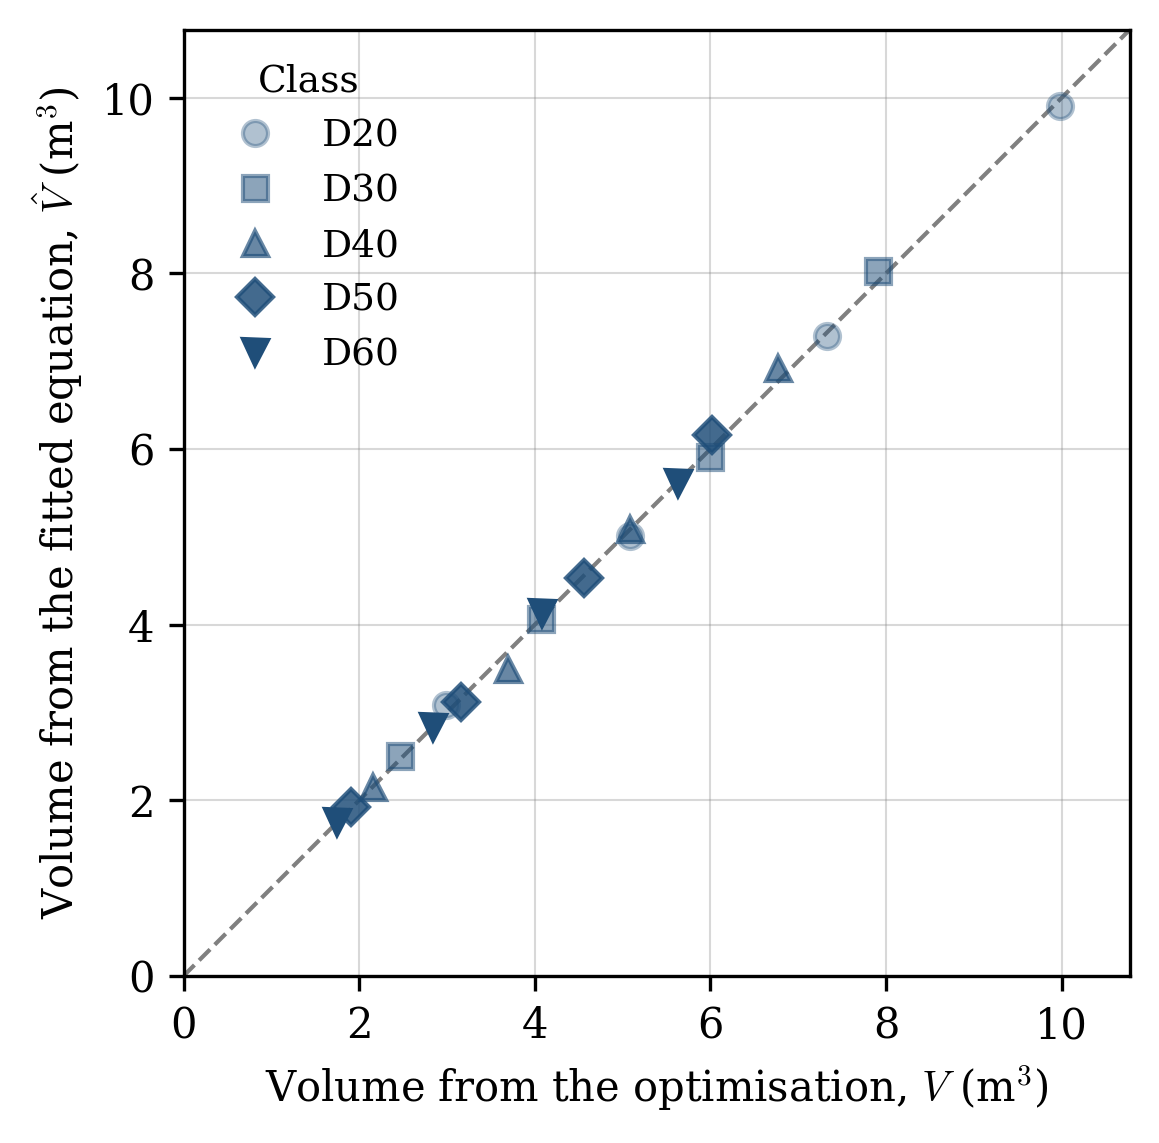
\includegraphics[width=0.4\textwidth]{figuras/en/equacao_pre_dimensionamento.png}
    \caption{Volume estimated by the pre-sizing equation (Eq.~\eqref{eq:pre_dimensionamento}) against the volume obtained by optimization, for the twenty cells of the matrix.}
    \label{fig:equacao_pre_dimensionamento}
\end{figure}

The error is not concentrated in any identifiable subset of the matrix. Since Section~\ref{sec:varredura} showed that none of the twenty cells saturates at the dimensional lower bound of the search domain, Eq.~\eqref{eq:pre_dimensionamento} does not suffer here from the limitation, common to fits of this kind, of ignoring a side constraint of the algorithm. The maximum error of 5.32\%, in cell C-08, reflects only the expected residual of a three-parameter fit over twenty observations, with no discernible relationship with the span or class of the cell.
The signs of the fitted exponents have a direct physical reading and reinforce the consistency of the model with Section~\ref{sec:varredura}. The value $b = 1.683 > 1$ reproduces the same feedback between self-weight and section that produces exponents $n$ between 1.64 and 1.73 per class, and $c = -0.518 < 0$ expresses that increasing $f_{c0,k}$ reduces the required volume, as expected.
The exponent $b$ of the joint equation indeed lies within the range of exponents $n$ observed class by class, which indicates that tying the five curves into a single continuous surface in $f_{c0,k}$ does not distort the behaviour already identified for each class separately.

To verify the interpolation capability of Eq.~\eqref{eq:pre_dimensionamento} outside the fitting set, two additional configurations with intermediate spans not belonging to the matrix were optimized, $L = 4.5$~m with class D30 and $L = 5.5$~m with class D50, keeping all other parameters of Table~\ref{tab:parametros} and of the algorithm (Table~\ref{tab:nsga2}) unchanged.
Neither of these two solutions took part in fitting the coefficients $a$, $b$ and $c$.
Table~\ref{tab:validacao_equacao} compares the volume of the minimum volume solution obtained by optimization with the volume predicted by the equation.

\begin{table}[!ht]
\caption{Verification of the pre-sizing equation at intermediate spans not used in the fit.\label{tab:validacao_equacao}}
\begin{threeparttable}
\begin{tabular*}{\columnwidth}{@{\extracolsep\fill}ccccc@{\extracolsep\fill}}
\toprule
$L$ (m) & Class & $V$ optimization (m\textsuperscript{3}) & $\hat{V}$ equation (m\textsuperscript{3}) & Relative error \\
\midrule
4.5 & D30 & 4.969 & 4.944 & $-0.52\%$ \\
5.5 & D50 & 5.395 & 5.319 & $-1.42\%$ \\
\bottomrule
\end{tabular*}
\begin{tablenotes}
\footnotesize
\item Optimizations with $\rho = 5\%$ and the same parameters as the twenty cells of the matrix. The relative error is $(\hat{V} - V)/V$.
\end{tablenotes}
\end{threeparttable}
\end{table}

The two errors, of $-0.52\%$ and $-1.42\%$, are of the same order of magnitude as the mean error obtained over the fitting cells, and the optimized volumes lie between those of the neighbouring cells of the matrix with the same class (4.076 and 6.001~m\textsuperscript{3} for D30 between 4 and 5~m, and 4.562 and 6.015~m\textsuperscript{3} for D50 between 5 and 6~m).
In both configurations girder bending is the governing check, in line with the behaviour observed in Section~\ref{sec:varredura}.
This result indicates that the equation interpolates consistently between the tabulated spans, without, however, authorizing its use outside the investigated domain.
